
\documentclass[a4paper]{article}
\usepackage{graphicx}

\begin{document}

\section{Introduction}
This document describes how the problem of 2d-navigation was solved on a real robot.
The goal of navigation is to safely move a robot from a to b. The robot used
was moving base, the x80sv.


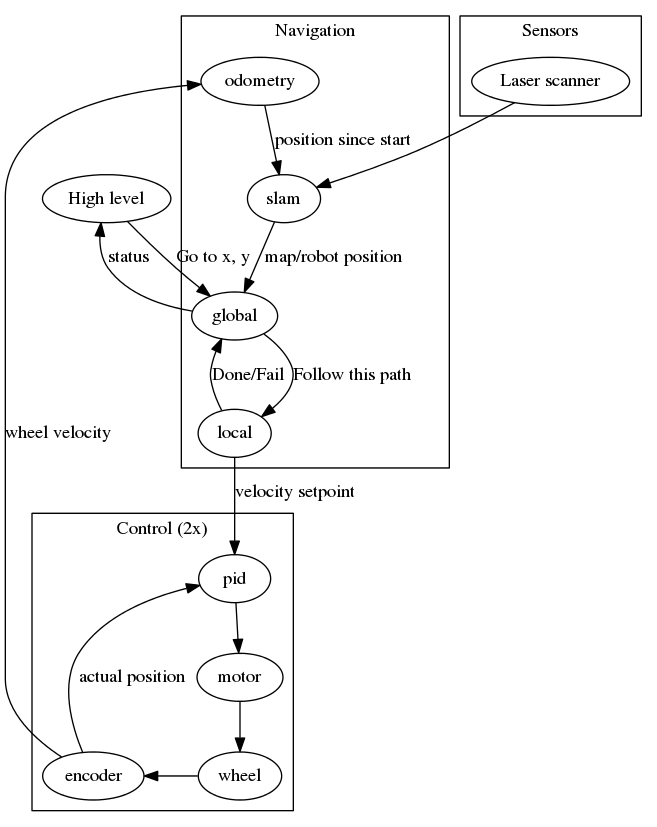
\includegraphics[width=\textwidth,height=\textheight,keepaspectratio]{img/overview.png}

The task of navigation can be split up into the following tasks:

\begin{itemize}
  \item Robot control. This task is concerned with controlling the seperate wheels of the robot. Typically this is done using PID control or something alike.
  \item Odometry calculation. By keeping track of wheel motions, the robot position can be
calculated. This method is subjective to drift.
  \item Position and mapping, also known as SLAM, is the task of determining location of the robot in the world, and at the same time reconstructing the world.
  \item Global planning is the task of determining a path through a known map. This requires a search like A* or something like that.
  \item Local planning takes as input the global path and generated the appropriate motion commands for the robot control. It is some sort of setpoint generator. This layer is also responsible for obstacles. When an obstacle is observed, the path may be adjusted.
\end{itemize}

The rest of this document describes all the tasks listed above as applied to the x80sv using the robot operating system (ROS).

\section{Installation}


\section{Navigation}

\section{Options}

\section{Odometry}

\section{slam}

\end{document}

